\documentclass[professionalfonts]{beamer}
\usepackage[familydefault,light]{Chivo} 
\usepackage[T1]{fontenc}
\usenavigationsymbolstemplate{}
\usepackage[]{hyperref}
\usepackage{tikz,pgf,pgfarrows,pgfnodes,pgfbaseimage}
\graphicspath{{./Pics/}}
\usetikzlibrary{shapes}
\usepackage{setspace}
\newcommand{\evi}[1]{{\colorbox{yellow!50}{{#1}}}}
\newcommand{\exe}[1]{{\color{black!50}{{#1}}}}
\newcommand{\kw}[1]{{\colorbox{black!30}{\color{white}{#1}}}}
\tikzstyle{nd}=[circle,draw=black,thick,minimum size=.8cm,inner sep=1pt]
\setbeamercovered{transparent}
\usetheme{Singapore}
\tikzstyle{nodo}=[ellipse,draw=black!60,fill=black!10,line width=.7pt,minimum width=.7cm,minimum height=.4cm]
\usecolortheme[named=gray]{structure}
\setbeamercolor{block title}{bg=black!20,fg=black}
\setbeamercolor{block body}{bg=black!10,fg=black}

\title{Algoritmi Numerici}
\subtitle{Introduzione al corso}
\author{Alessandro Antonucci\\{\tt alessandro.antonucci@supsi.ch}}
\date{Anno Accademico 2019 - 2020}
%%%%%%%%%%%%%%%%%%%%%%%%%%%%
\begin{document}
\maketitle
\frame{\frametitle{Il corso}
\setstretch{1.4}
\begin{itemize}
\item 6 ECTS
\item Ore settimanali: 2 (teoria) + 2 (esercitazioni)\\entrambi i semestri
\item Docente: Alessandro Antonucci\\
{\tt email: alessandro.antonucci@supsi.ch}\\
{\tt skype: alessandro.antonucci}\\
{\tt web: \href{http://www.idsia.ch/~alessandro}{www.idsia.ch/$\sim$alessandro}}
\item Esercitazioni: Lorenzo Camponovo + Lilith Mattei\\(+ Antonucci)
\end{itemize}}

\frame{\frametitle{Orario}
\begin{center}
\includegraphics[width=6cm,height=6cm]{orario}
\end{center}}

\frame{\frametitle{Contenuti e prove scritte}
\vskip 2mm
\setstretch{1.3}
\begin{tabular}{ll}
{\small set-nov}&\colorbox{yellow!50}{Rappresentazioni del numero}\\
{\small nov-gen}& Risoluzione equazioni non-lineari\\
{\small feb-apr}& Risoluzione di sistemi di equazioni lineari\\
{\small apr-giu}& Interpolazione ed integrazione numerica 
\end{tabular}
\begin{center}
\vskip 5mm
Una prova scritta per ogni semestre (note $\{n_i\}_{i=1}^2$)

\begin{itemize}
\item $\min_{i=1,2} n_i \geq 6$ (ambizioso)
\item $(n_1\geq 4) \wedge (n_2\geq 4) $ (dignitoso)
\item $\sum_{i=1}^2 n_i \geq 8$ (minimale)
\end{itemize} 
\vskip 5mm
Durante la prova scritta a disposizione\\2 fogli A4 (fronte retro) con appunti
\end{center}
}

\frame{\frametitle{Scopo del Corso}
\begin{columns}
\begin{column}[T]{0.5\textwidth}
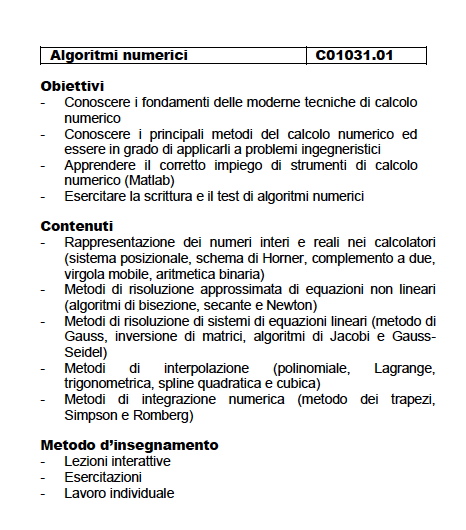
\includegraphics[width=6cm]{Piano}
\end{column}
\begin{column}[T]{0.5\textwidth}
\vskip 5mm
Come da piano di studio
\vskip 5mm
Ma anche:
\begin{itemize}
\item Formalizzare problemi in maniera algoritmica
\item Gestire complessit\`a tecnica nei calcoli
\item ``Svelare'' questioni legate alla rappresentazione dei numeri ed alla risoluzione di problemi mediante calcolatore
\end{itemize}
\end{column}
\end{columns}
}

\frame{\frametitle{Presenze}
\setstretch{1.3}
\begin{itemize}
\item Presenze rilevate online all'inizio di ogni lezione
\item In caso di assenza mandare una mail al docente\\(se possibile prima della lezione)
\item E-mail {\tt @student.supsi.ch} = strumento di comunicazione col docente
\item Inizio e fine dalla lezione col suono della campanella
\item No ritardi ingiustificati
\end{itemize}}

\frame{\frametitle{Tools}
\setstretch{1.3}
\begin{itemize}
\item Studenti iscritti al modulo su {\tt\href{http://www.icorsi.ch}{icorsi.ch}} dal docente
\item Materiali disponibili sulla piattaforma 
\item Forum per domande/discussioni
\item Strumenti software: iPython, Java, Excel, Geogebra, Kahoot, $\ldots$ 
\item Cartella Dropbox/Owncloud/Git/Colab condivisa per codice
\end{itemize}}
\end{document}
